%% stim-u55c paper -- Journal of Supercomputing submission
%% Springer Nature LaTeX template (sn-jnl.cls), sn-basic reference style.
%% Self-contained: compiles with pdflatex directly in this folder / on Overleaf.

\documentclass[pdflatex,sn-basic]{sn-jnl}

\usepackage{graphicx}
\usepackage{multirow}
\usepackage{amsmath,amssymb,amsfonts}
\usepackage{amsthm}
\usepackage{mathrsfs}
\usepackage[title]{appendix}
\usepackage{xcolor}
\usepackage{textcomp}
\usepackage{manyfoot}
\usepackage{booktabs}
\usepackage{algorithm}
\usepackage{algorithmicx}
\usepackage{algpseudocode}
\usepackage{listings}
\usepackage{url}

\raggedbottom

\begin{document}

\title[stim-u55c]{stim-u55c: An FPGA-Accelerated, Stim-Compatible Pauli Frame Sampler for Stabilizer Quantum Error-Correction Circuits on the AMD Alveo U55C}

\author*[1]{\fnm{Nasir} \sur{Ali}}\email{nasirali2607@gmail.com}

\affil*[1]{\orgname{Centre for Development of Advanced Computing (C-DAC)}, \orgaddress{\city{Noida}, \country{India}}}

\abstract{Monte Carlo sampling of stabilizer quantum error-correction (QEC) circuits -- generating large numbers of independent detector-event shots for decoder benchmarking, threshold estimation, and logical-error-rate characterization -- is a recurring computational bottleneck in QEC research, and is addressed almost exclusively on CPUs by existing tools. This paper presents stim-u55c, a Stim-compatible Pauli frame sampler and detector sampler implemented as a Vitis High-Level Synthesis (HLS) kernel and deployed on an AMD/Xilinx Alveo U55C FPGA accelerator card. The system compiles a stabilizer circuit and its error model ahead of time into a compact instruction stream, resolving detector- and observable-folding masks at compile time rather than runtime, and executes it on a counter-based (Philox4x32-10) hardware sampler. We validate the design with a five-tier methodology -- noiseless determinism, bit-exact agreement with a Python reference model, single-fault injection against the circuit's detector error model, statistical equivalence with Stim at scale, and PyMatching-decoded logical error rate -- first in software and cosimulation, then end-to-end on physical Alveo U55C hardware. We report, in full and without adjustment, the empirical gap between Vitis HLS's own resource and frequency estimates and the real post-place-and-route result (post-route LUT usage 2.6$\times$ lower than HLS estimated, yet timing closure required five real implementation attempts and just over 20 hours of cumulative build time), and an honest throughput comparison in which the current, unpipelined kernel is outperformed by single-core CPU Stim by 5.6$\times$--15.3$\times$ depending on circuit size, with the two architectural causes identified and quantified. All code, build scripts, and raw results are publicly available.}

\keywords{FPGA acceleration, quantum error correction, stabilizer circuit simulation, Pauli frame propagation, High-Level Synthesis, Alveo U55C, Monte Carlo sampling, surface codes}

\maketitle

\section{Introduction}\label{sec1}

Simulating and sampling from stabilizer quantum error-correction circuits is central to QEC research: estimating a code's threshold, benchmarking a decoder, or characterizing a logical error rate all require drawing very large numbers of independent syndrome samples (``shots'') from a noisy circuit and, for a fraction of validation work, decoding them. Stim~\cite{gidney2021stim} made this workload tractable on CPUs by simulating stabilizer circuits in the Pauli-frame representation rather than by full tableau propagation~\cite{gottesman1998heisenberg,aaronson2004chp}: instead of tracking the exact stabilizer group through every gate, a Pauli frame simulator tracks only how noise deviates from a fixed, noiseless reference execution, which turns each shot into an inexpensive, bit-packed, embarrassingly parallel update. Stim's own implementation exploits this with heavily vectorized (SIMD) CPU code, and its documentation notes that the fine-grained, bit-packed nature of the workload makes further parallelization -- in particular naive GPU offload -- less rewarding than the shot count alone would suggest, since each shot's per-gate update is memory-bandwidth-bound and low in arithmetic intensity rather than compute-bound.

This motivates asking whether a different class of hardware -- an FPGA, with its ability to instantiate a custom, deeply pipelined, bit-level datapath rather than relying on a general-purpose SIMD/SIMT execution model -- can accelerate this same workload, and, just as importantly, whether the answer can be established honestly: by building the whole pipeline, from circuit compilation through real silicon, and reporting what a careful, staged validation process actually finds, including where it falls short.

This paper presents \textbf{stim-u55c}, an FPGA-accelerated, Stim-compatible Pauli frame sampler and detector sampler implemented as a Vitis HLS kernel and deployed on an AMD/Xilinx Alveo U55C data-center accelerator card. The contributions are:

\begin{itemize}
\item A compile-time instruction-stream architecture for Pauli frame sampling that resolves gate scheduling, detector folding, and observable folding ahead of time, so the FPGA kernel itself needs no runtime measurement-history bookkeeping (Section~\ref{sec:arch}).
\item A five-tier validation methodology -- noiseless determinism, bit-exact agreement with a software oracle, single-fault-injection agreement with the circuit's detector error model (DEM), large-sample statistical equivalence with Stim, and PyMatching-decoded logical-error-rate agreement -- applied first in software and RTL cosimulation and then, unmodified, on real hardware (Section~\ref{sec:validation}).
\item A full account of moving this design through real Vivado place-and-route, including a quantified, five-attempt timing-closure process and a direct, honest comparison between Vitis HLS's own \texttt{csynth\_design} resource and frequency estimates and what the real post-route implementation produced (Section~\ref{sec:results}).
\item An unembellished throughput result: the current kernel, in its present, not-yet-fully-pipelined form, is slower than single-core CPU Stim, and we identify and quantify the two specific architectural reasons why, as concrete targets for future work (Sections~\ref{sec:results} and~\ref{sec:discussion}).
\end{itemize}

Every quantitative result in this paper is drawn directly from the project's own committed build logs and benchmark output, all of which are publicly available alongside the source code (Section~\ref{sec:availability}).

\section{Background and Related Work}\label{sec2}

\subsection{Stabilizer circuits and Pauli frame simulation}

Stabilizer circuits -- built from Clifford gates and Pauli measurements -- underlie essentially every practical QEC code, including the surface code~\cite{kitaev2003faulttolerant,dennis2002topological,fowler2012surface}. The Gottesman--Knill theorem allows such circuits to be simulated efficiently classically, and the tableau method of Aaronson and Gottesman~\cite{aaronson2004chp} (building on Gottesman's Heisenberg-picture formalism~\cite{gottesman1998heisenberg}) does so by explicitly tracking how the stabilizer group evolves. Stim~\cite{gidney2021stim} instead simulates a \emph{Pauli frame}: a fixed, noiseless reference trajectory is computed once, and each sampled shot only tracks the accumulated deviation (an X/Z Pauli frame per qubit) introduced by that shot's random noise draws, propagated forward through the same gate sequence and finally folded into detector and observable outcomes. This turns per-shot simulation into simple, bit-packed XOR/AND updates that vectorize well and require no shot-to-shot dependent state, which is exactly the property stim-u55c exploits to move the same update rule into fixed hardware.

\subsection{Decoding as a separate, downstream problem}

Stabilizer sampling and decoding are separate problems joined only by the detector error model (DEM). This paper's software and hardware validation both use PyMatching's Sparse Blossom minimum-weight perfect matching implementation~\cite{higgott2023sparseblossom} purely as a correctness \emph{oracle} -- to confirm sampled syndromes decode to the logical error rate an independently-generated, CPU-sampled syndrome stream would -- not as something reimplemented on the FPGA. Decoding hardware acceleration is its own active research area, with FPGA and ASIC decoders including lookup-table-based decoders for small codes~\cite{das2022lilliput}, distributed/parallel Union-Find implementations reaching large code distances~\cite{liyanage2023fpgadecoder,delfosse2021unionfind}, and real-time matching-based decoders demonstrated at the scale of hundreds to low thousands of physical qubits~\cite{barber2023realtime}. stim-u55c is complementary to this line of work: it accelerates the \emph{generation} of syndromes for offline threshold estimation and decoder benchmarking, a workload with different throughput/latency requirements than online, per-round decoding.

\subsection{Counter-based random number generation}

Each simulated shot needs its own, reproducible stream of noise draws. stim-u55c uses the Philox4x32-10 counter-based generator~\cite{salmon2011parallel}: because a Philox output depends only on a key and a counter, with no sequential state to carry between draws, arbitrarily many independent streams can be instantiated in parallel hardware lanes and reseeded per shot for free, which suits an FPGA datapath far better than a state-carrying generator would.

\section{System Architecture}\label{sec:arch}

\subsection{Pipeline overview}

Figure~\ref{fig:arch} shows the end-to-end pipeline. On the host, a \texttt{stim.Circuit} and its noise parameters are compiled (\texttt{kernel/isa.py}) into a flat, un-broadcast instruction stream: every Clifford gate, measurement, and noise-injection opcode in the circuit becomes one instruction, with per-qubit and per-shot broadcasting resolved at compile time rather than left for the kernel to unpack at runtime. That instruction stream is transferred once over PCIe via the Xilinx Runtime (XRT)~\cite{amd_xrt}, after which the FPGA kernel executes it repeatedly, once per launch, each launch sampling a batch of shots in parallel hardware lanes. Detector- and observable-folded output leaves the device bit-packed, one 64-bit word per detector (bit $s$ = shot $s$'s outcome), and is decoded or statistically compared on the host.

\begin{figure}[h]
\centering
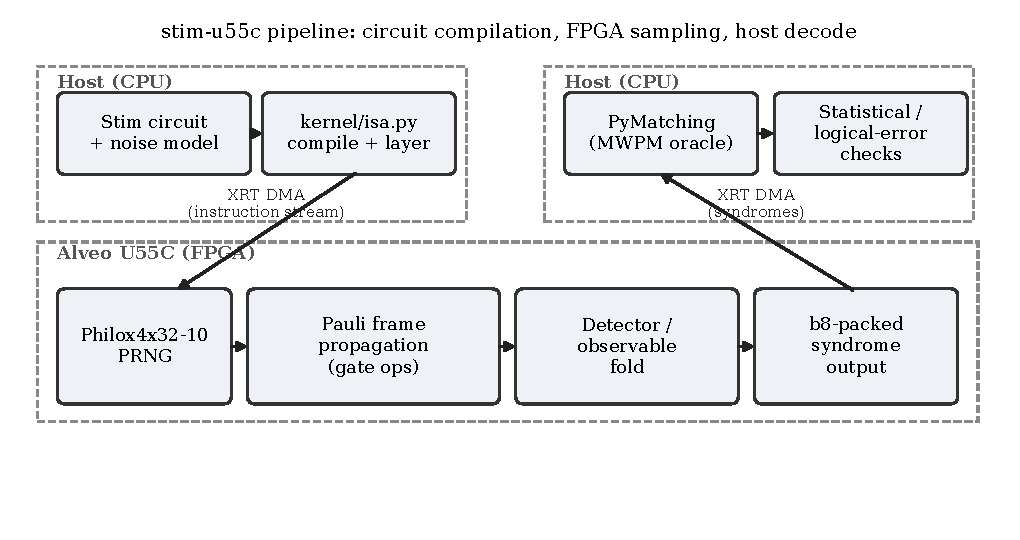
\includegraphics[width=\textwidth]{figures/architecture.pdf}
\caption{stim-u55c pipeline: circuit compilation on the host, Pauli frame propagation and detector/observable folding on the Alveo U55C, decoding and validation back on the host.}
\label{fig:arch}
\end{figure}

\subsection{Instruction set and Pauli frame representation}

Each qubit's Pauli frame is held as an (X, Z) bit pair per shot lane. Single- and two-qubit Clifford gates are compiled to fixed update rules over these bit pairs (e.g. Hadamard swaps a qubit's X and Z frame bits; CNOT propagates both qubits' frame bits according to the standard stabilizer update table); measurement instructions read a qubit's frame bit, XOR it against the corresponding noiseless reference outcome computed at compile time, and route the result toward the detectors and observables that depend on it. Noise instructions draw from the per-shot-lane Philox generator and flip frame bits according to the circuit's declared error channels (depolarizing, Pauli, etc.).

\subsection{Compile-time detector and observable folding}

A na\"ive hardware implementation would need a runtime measurement-history buffer so that each detector -- defined as an XOR of a specific subset of prior measurement outcomes -- could be resolved once all its constituent measurements have occurred. stim-u55c avoids this: because the circuit and its detector/observable definitions are fully known at compile time, \texttt{encode\_circuit} precomputes, for every measurement instruction, the compile-time-resolved fold mask identifying which detector and/or observable accumulators it contributes to. The kernel then only ever needs a small, fixed set of live accumulator registers, folded incrementally as measurements occur, with no runtime history lookup or dynamic indexing.

\subsection{Instruction layering}

Reordering mutually qubit-disjoint instructions into layers lets independent instructions execute back-to-back without a Pauli-frame data hazard, a prerequisite for pipelining the per-instruction execution loop. \texttt{kernel/isa.py:\_layer\_and\_reorder} implements this as the last compilation step, and a Python-side check confirms no two instructions scheduled into the same layer share a qubit, for every circuit used in this paper. Because the reordering only ever changes an instruction's own Philox counter value -- never which qubit sees which effect, or their relative order along a given qubit -- the bit-exact validation of Section~\ref{sec:validation} (Tier 2) confirms the reordering is semantically transparent. Table~\ref{tab:layering} gives layering statistics for the three circuits used throughout this paper.

\begin{table}[h]
\caption{Instruction-layering statistics: qubit-disjoint layers computed by \texttt{\_layer\_and\_reorder} for each circuit.}\label{tab:layering}
\begin{tabular}{@{}lrrr@{}}
\toprule
Circuit & Instructions & Layers & Avg.\ instructions/layer \\
\midrule
Repetition code, $d=3$ & 45 & 14 & 3.2 \\
Surface code, $d=3$ & 344 & 47 & 7.3 \\
Surface code, $d=5$ & 1{,}674 & 77 & 21.7 \\
\botrule
\end{tabular}
\end{table}

Layering alone was not sufficient to reach a fully pipelined (initiation interval, II$=1$) instruction loop; Section~\ref{sec:discussion} reports why, and quantifies the II attempt that was made and reverted.

\subsection{Counter-based noise generation}

Every noise draw uses a 10-round Philox4x32 instance~\cite{salmon2011parallel}, keyed per shot lane so that lanes never share PRNG state. The kernel originally instantiated two textually distinct Philox-drawing functions for two different noise-consumption patterns (a flip-mask draw and a categorical-outcome draw); because the two functions were textually different despite being mutually exclusive within any single instruction, Vitis HLS had no basis to share hardware between them. Merging them into one \texttt{draw\_noise} function let HLS's ordinary mutually-exclusive-branch resource sharing consolidate the two Philox banks into one -- a resource-usage finding reported quantitatively in Section~\ref{sec:results}.

\section{Validation Methodology}\label{sec:validation}

Correctness for a hardware-accelerated stabilizer sampler cannot be established by a single check: an instruction-encoding bug, a detector-folding bug, and a systematic statistical bias would each need a different kind of test to surface. stim-u55c therefore validates through five progressively stronger tiers, applied identically at every implementation stage (Python reference model, C simulation, RTL cosimulation, hardware emulation, and finally real hardware) so that a failure at any stage localizes to what changed since the last passing stage.

\begin{description}
\item[Tier 1 -- Noiseless determinism.] With all noise channels disabled, every detector and observable must be exactly zero (a noiseless stabilizer circuit's detectors never fire by construction). This is the cheapest possible check and catches gross frame-propagation or folding errors immediately.
\item[Tier 2 -- Bit-exact agreement with a software oracle.] Kernel output must match, bit-for-bit, a from-scratch Python reference sampler (\texttt{softmodel/reference\_sampler.py}) driven by the identical PRNG stream, for every shot and every detector/observable.
\item[Tier 3 -- Single-fault injection vs.\ the DEM.] For every mechanism in the circuit's Stim-generated detector error model, a circuit with exactly that one fault forced (probability 1, all other noise disabled) is compiled and sampled; the resulting detector/observable pattern must match the DEM mechanism's own symptom exactly. This directly tests whether the compiled instruction stream's detector-folding topology matches the DEM Stim itself derived from the same circuit.
\item[Tier 4 -- Statistical equivalence with Stim at scale.] At realistic noise levels and shot counts ($10^6$--$10^7$), per-detector and per-observable firing rates from the kernel must agree with Stim's own sampler within a $5\sigma$ two-proportion $z$-test bound.
\item[Tier 5 -- Logical error rate via PyMatching.] Real, decoded logical error rates from kernel-sampled syndromes must agree, within the same $5\sigma$ bound, with logical error rates from independently CPU-sampled syndromes decoded by the identical PyMatching matcher -- the end-to-end check that ties syndrome correctness to the quantity a QEC study actually cares about.
\end{description}

Three circuits are used throughout: a distance-3 repetition code, and distance-3 and distance-5 rotated surface codes (memory experiments), the largest distances the kernel's compile-time qubit budget ($\mathrm{NUM\_QUBITS\_MAX}=128$) supports without a fresh synthesis run.

\section{Implementation}\label{sec:impl}

The kernel (\texttt{kernel/stim\_frame\_sampler.cpp}) is written as \texttt{extern "C"} Vitis HLS C++, synthesized with Vitis HLS 2023.2 for the Alveo U55C's target part (\texttt{xcu55c-fsvh2892-2L-e}, platform \texttt{xilinx\_u55c\_gen3x16\_xdma\_3\_202210\_1}) and linked into an \texttt{xclbin} with \texttt{v++}. The same source compiles, via a thin C-simulation shim, as ordinary C++ for fast, toolchain-free CI testing, so unit and Tier 1--4 tests run on every change without requiring the vendor toolchain.

The host runtime uses XRT directly (four small C++ tools under \texttt{host/}: single-shot correctness checking, a double-buffered throughput benchmark, and double-buffered Tier 4/Tier 5 variants that accumulate or transpose output across many launches respectively). Mode A throughput execution keeps two \texttt{xrt::run} objects in flight so that host-side setup for launch $i{+}1$ overlaps device execution of launch $i$, avoiding the per-process \texttt{xclbin} reload cost that would otherwise dominate any repeated-launch measurement.

\section{Results}\label{sec:results}

\subsection{Software validation}

All five tiers pass in software before any hardware synthesis is attempted: the project's pytest suite (18 tests covering Tiers 1, 3, and 4 against the Python reference model, plus unit testbenches for the PRNG and gate-operation logic, plus a C-simulation Tier 2 bit-exactness check for all three circuits) passes in full, in 129.5 seconds.

\subsection{HLS synthesis estimate vs.\ real post-route implementation}

Table~\ref{tab:resources} and Figure~\ref{fig:resources} compare Vitis HLS's own \texttt{csynth\_design} resource and frequency estimate (Phase-3 gate, target 300\,MHz) against the real, timing-closed post-place-and-route result. The Philox merge described in Section~\ref{sec:arch} is the single largest contributor to the HLS-estimated numbers shown: before merging the two Philox-drawing functions into \texttt{draw\_noise}, HLS estimated 361{,}185 LUTs and 1{,}920 DSPs (83\% of one SLR's LUT budget); after merging, with no change to the frame, gate, or detector-fold logic, the estimate dropped to the 217{,}052 LUT / 960 DSP figures in the table.

\begin{table}[h]
\caption{Resource utilization: Vitis HLS's \texttt{csynth\_design} estimate (Phase 3, post-Philox-merge) vs.\ the real, timing-closed post-place-and-route implementation. HLS percentages are relative to one SLR / the full part, as HLS estimates against the SLR the kernel is bound to; post-route percentages are relative to the full device.}\label{tab:resources}
\begin{tabular}{@{}lrrrr@{}}
\toprule
Resource & HLS estimate & \% SLR (HLS) & Post-route & \% device (post-route) \\
\midrule
LUT & 217{,}052 & 49\% & 83{,}843 & 7.09\% \\
FF/Register & 174{,}517 & 20\% & 101{,}402 & 4.15\% \\
DSP & 960 & 31\% & 708 & 7.85\% \\
BRAM\_18K & 66 & 4\% & 21 & 1.16\% \\
\botrule
\end{tabular}
\end{table}

\begin{figure}[h]
\centering
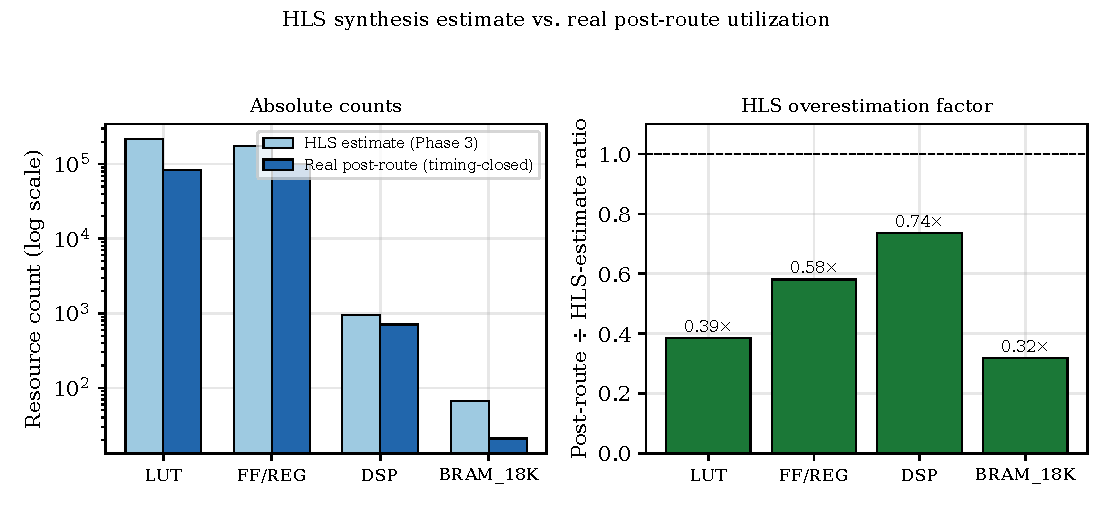
\includegraphics[width=\textwidth]{figures/resource_estimate_vs_real.pdf}
\caption{Left: absolute resource counts, HLS estimate vs.\ real post-route implementation (log scale). Right: post-route-to-HLS-estimate ratio per resource class -- HLS overestimates every resource class, most severely BRAM\_18K (3.1$\times$) and LUT (2.6$\times$).}
\label{fig:resources}
\end{figure}

Post-route LUT usage is $\sim$2.6$\times$ \emph{lower} than HLS's own estimate. This is a useful, concrete data point for anyone treating a \texttt{csynth\_design} report as a reliable predictor of final resource usage: it is a conservative upper bound from HLS's own RTL generation and mutually-exclusive-branch sharing analysis, not a substitute for what Vivado's real technology mapping, retiming, and logic optimization ultimately produce.

\subsection{Timing closure on real hardware}\label{sec:timing}

HLS's Fmax estimate (382.44\,MHz) proved considerably more optimistic than real timing closure at 250\,MHz: the design under-performed relative to the estimate to the point of taking five real \texttt{v++}/Vivado implementation attempts to close. Table~\ref{tab:timing} and Figure~\ref{fig:timing} summarize all five; every attempt failed at the same physical location -- placement- and routing-density around the replicated (64 shot lanes) Philox instances inside \texttt{draw\_noise} -- with the specific failing net changing between attempts (a divider, then a multiplier) even as the region stayed constant.

\begin{table}[h]
\caption{Real hardware ( \texttt{v++}/Vivado) timing-closure attempts. WNS = worst negative slack; a positive or zero WNS means all constraints are met.}\label{tab:timing}
\begin{tabular}{@{}clrrl@{}}
\toprule
\# & Configuration & WNS (ns) & Failing endpoints & Build time \\
\midrule
1 & 300\,MHz target, default directives & $-0.688$ & 26{,}495 & 3h\,53m \\
2 & ``250\,MHz'' (flag misapplied to \texttt{v++ -c} only) & $-1.092$ & 40{,}302 & 3h\,18m \\
3 & 250\,MHz target, correctly applied to \texttt{-c} and \texttt{-l} & $-0.179$ & 10{,}707 & 3h\,14m \\
4 & + \texttt{ExtraTimingOpt} / \texttt{AggressiveExplore} directives & $-0.041$ & 1{,}211 & 5h\,33m \\
5 & + \texttt{NoTimingRelaxation} (route) / post-route phys.\ opt. & $\mathbf{0.000}$ & \textbf{0} & 4h\,19m \\
\botrule
\end{tabular}
\end{table}

\begin{figure}[h]
\centering
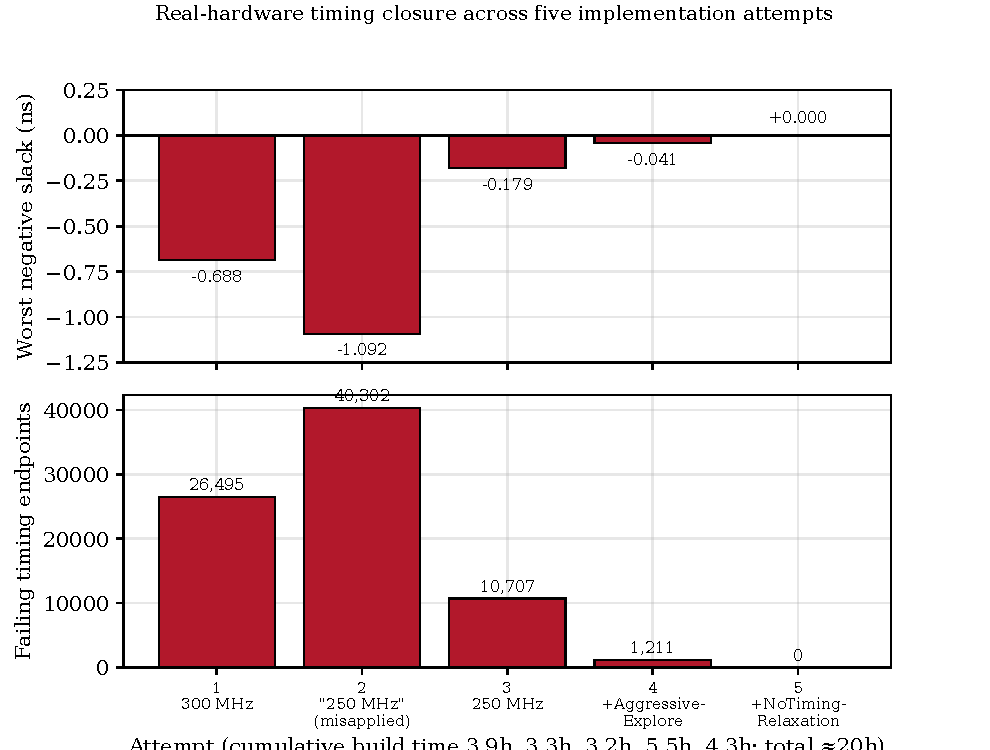
\includegraphics[width=\textwidth]{figures/timing_closure.pdf}
\caption{Worst negative slack and failing timing endpoints across the five real-hardware implementation attempts. Attempt 5 (\texttt{ROUTE\_DESIGN.ARGS.DIRECTIVE=NoTimingRelaxation} plus a post-route physical-optimization pass) closes timing completely.}
\label{fig:timing}
\end{figure}

Attempt 2 is included deliberately: it is a build that appeared to target 250\,MHz but, because the frequency flag was passed only to the \texttt{v++} compile stage and not the link/implementation stage, was actually still implemented at the original 300\,MHz clock period -- discovered only by checking the routed design's reported clock period directly rather than trusting the invoking script's intent. Attempt 5's fix, \texttt{ROUTE\_DESIGN.ARGS.DIRECTIVE=NoTimingRelaxation} together with an added \texttt{POST\_ROUTE\_PHYS\_OPT\_DESIGN} pass (also with an aggressive-exploration directive), fully closed timing: ``All user specified timing constraints are met.'' Cumulative real Vivado implementation time across all five attempts was just over 20 hours.

\subsection{Full-stack validation on real hardware}

All five validation tiers of Section~\ref{sec:validation} were re-run, unmodified, against the timing-closed bitstream on a physical Alveo U55C. Table~\ref{tab:hwvalidation} summarizes the results.

\begin{table}[h]
\caption{Five-tier validation results on real Alveo U55C hardware (not emulation).}\label{tab:hwvalidation}
\begin{tabular}{@{}p{0.6cm}p{4.4cm}p{3.6cm}p{4.1cm}@{}}
\toprule
Tier & What & Circuits & Result \\
\midrule
1 & Noiseless determinism & rep $d{=}3$, surface $d{=}3$, surface $d{=}5$ & \textbf{PASS} -- all detector/observable words exactly zero, all 64 shot lanes \\
2 & Bit-exact vs.\ soft model & rep $d{=}3$, surface $d{=}3$, surface $d{=}5$ & \textbf{PASS} \\
3 & Single-fault injection vs.\ DEM & rep $d{=}3$, surface (Z) $d{=}3$, surface (X) $d{=}3$ & \textbf{PASS} -- 458/458 DEM error mechanisms, $\sim$92\,s \\
4 & Statistical equivalence vs.\ CPU Stim & rep $d{=}3$, surface $d{=}3$, surface $d{=}5$ & \textbf{PASS} -- $10^7$ shots/circuit, max$|z|$ = 1.64 / 2.91 / 2.64, $\sim$6m\,42s total \\
5 & Logical error rate vs.\ Stim+PyMatching & surface $d{=}3$, surface $d{=}5$ & \textbf{PASS} -- 6 points (2 distances $\times$ 3 error rates), max$|z|$ = 1.59 \\
\botrule
\end{tabular}
\end{table}

Tier 3's fault-injection circuits are built by walking a Stim \texttt{CircuitErrorLocation}'s stack frames and flipped-Pauli product with the same path-matching logic already used (and separately validated) to \emph{interpret} a fault, but emitting an actual \texttt{stim.Circuit} with an explicit, forced single-Pauli error instead -- so Tier 3 needs no fault-injection mode in the kernel or compiler; it runs through the ordinary, unmodified compilation and execution path.

Tier 5 required transposing the kernel's detector-major bit-packed output (one 64-bit word per detector) into PyMatching's shot-major \texttt{decode\_batch(bit\_packed\_shots=True)} convention on the host; this transpose was itself cross-checked against the independently-validated Tier 4 aggregate-popcount path on the same instruction stream and seed sequence (0 mismatches across all 8 detectors of the repetition-code circuit) before being trusted for hardware-time measurements. Table~\ref{tab:ler} and Figure~\ref{fig:ler} give the full Tier 5 result.

\begin{table}[h]
\caption{Tier 5: logical error rate, FPGA-sampled syndromes vs.\ CPU-Stim-sampled syndromes, both decoded with the identical PyMatching 2.4.0 matcher. Surface code, rotated memory Z, $10^6$ shots/point.}\label{tab:ler}
\begin{tabular}{@{}rrrrr@{}}
\toprule
$d$ & $p$ & FPGA LER & CPU Stim LER & $z$ \\
\midrule
3 & 0.0010 & 0.00074 & 0.00079 & $-1.38$ \\
3 & 0.0030 & 0.00651 & 0.00662 & $-0.93$ \\
3 & 0.0100 & 0.05906 & 0.05919 & $-0.40$ \\
5 & 0.0010 & 0.00013 & 0.00016 & $-1.59$ \\
5 & 0.0030 & 0.00331 & 0.00332 & $-0.06$ \\
5 & 0.0100 & 0.08412 & 0.08395 & $0.42$ \\
\botrule
\end{tabular}
\end{table}

\begin{figure}[h]
\centering
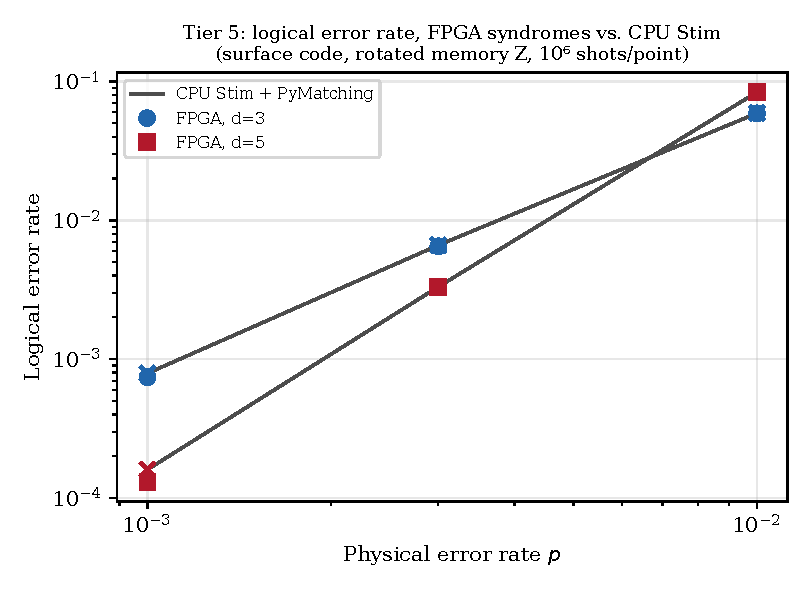
\includegraphics[width=0.75\textwidth]{figures/logical_error_rate.pdf}
\caption{Tier 5 logical error rate vs.\ physical error rate, FPGA-sampled ($\bigcirc$/$\square$) vs.\ CPU-Stim-sampled ($\times$) syndromes, $d=3$ and $d=5$. Below the apparent threshold ($p=0.001,0.003$) $d=5$ outperforms $d=3$; above it ($p=0.01$) the ordering reverses, the expected above/below-threshold signature, recovered from real hardware syndromes without being targeted.}
\label{fig:ler}
\end{figure}

The rates in Table~\ref{tab:ler} show the qualitative behavior a correctly functioning surface code should: below the apparent threshold, $d=5$ has a lower logical error rate than $d=3$ (error suppression with distance); at $p=0.01$, $d=5$ does worse than $d=3$, the classic above-threshold signature where a larger code has more opportunities to fail. This was not tuned for; it falls directly out of real hardware-sampled syndromes being decoded correctly. $d=7,9,11$ were not attempted: $d=7$ alone needs more qubits than the current kernel's $\mathrm{NUM\_QUBITS\_MAX}=128$ supports ($d=11$ needs 274), and given the timing-closure experience of Section~\ref{sec:timing}, extending the qubit budget carries a real risk of a further multi-attempt closure process at a larger, likely more resource-hungry design -- scoped, separate future work rather than something undertaken speculatively.

\subsection{Throughput}

Table~\ref{tab:throughput} and Figure~\ref{fig:throughput} report Mode A throughput (shots/second), FPGA at 250\,MHz vs.\ single-core CPU Stim (\texttt{compile\_detector\_sampler().sample(bit\_packed=True)}) on an AMD EPYC 7742. The FPGA measurement excludes one-time device/\texttt{xclbin} load but includes every subsequent launch's setup, execution, and DMA synchronization, with two \texttt{xrt::run} objects kept in flight (Section~\ref{sec:impl}); it reflects 5{,}000 launches per circuit at \texttt{SHOTS=64} shots/launch (320{,}000 shots total); the CPU baseline draws $2\times10^6$ shots per circuit.

\begin{table}[h]
\caption{Mode A throughput: FPGA (Alveo U55C, 250\,MHz) vs.\ single-core CPU Stim, same circuits.}\label{tab:throughput}
\begin{tabular}{@{}lrrr@{}}
\toprule
Circuit & FPGA (shots/s) & CPU Stim (shots/s) & CPU speedup \\
\midrule
Repetition code, $d=3$ & 865{,}117 & 4{,}867{,}590 & 5.6$\times$ \\
Surface code, $d=3$ & 160{,}104 & 2{,}260{,}033 & 14.1$\times$ \\
Surface code, $d=5$ & 33{,}587 & 512{,}610 & 15.3$\times$ \\
\botrule
\end{tabular}
\end{table}

\begin{figure}[h]
\centering
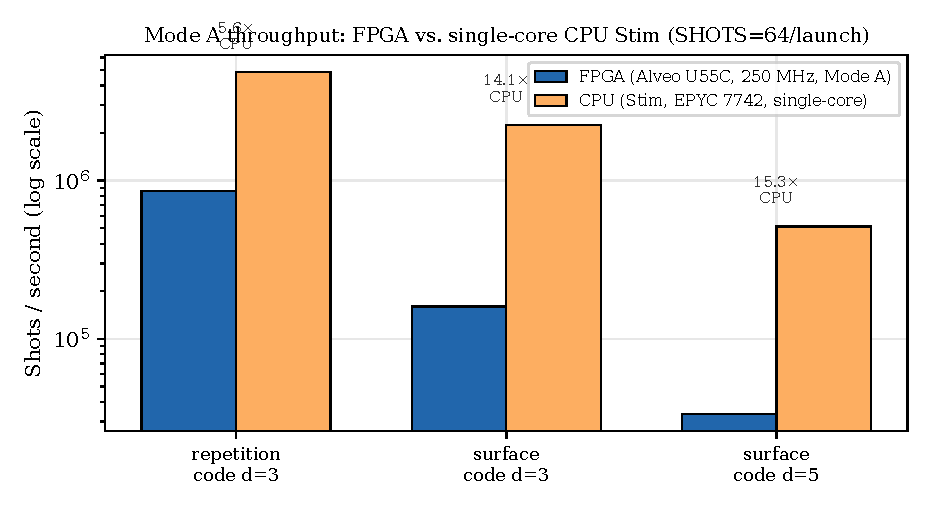
\includegraphics[width=0.75\textwidth]{figures/throughput.pdf}
\caption{Mode A throughput, FPGA vs.\ single-core CPU Stim, log scale. The current, unpipelined kernel is outperformed by CPU Stim at every circuit size tested; the gap widens with circuit size.}
\label{fig:throughput}
\end{figure}

CPU Stim outperforms the current FPGA implementation at every circuit size tested, and the gap widens with circuit size. Section~\ref{sec:discussion} identifies and quantifies the two specific, architectural reasons.

\section{Discussion}\label{sec:discussion}

\subsection{Why HLS estimates were unreliable in both directions}

The results above show HLS's own \texttt{csynth\_design} estimates being wrong in \emph{both} directions relative to reality, for different resources: resource usage was substantially overestimated (Section~\ref{sec:results}, up to 3.1$\times$ for BRAM\_18K), while achievable frequency was substantially overestimated too, in the sense that reaching a real, fully-closed 250\,MHz implementation -- well below the 382.44\,MHz HLS estimate at a 300\,MHz target -- took five real attempts and dedicated timing-closure engineering (aggressive placement/routing directives, a post-route physical-optimization pass) rather than following automatically from the RTL HLS generated. Both effects trace to the same root cause: \texttt{csynth\_design} estimates are produced from HLS's own RTL generation and a simplified timing model, not from Vivado's real technology mapping, placement, and routing, which is where physical effects like the routing-dominated (97.8\% of critical-path delay routing rather than logic in the worst attempt) congestion around the replicated Philox instances actually appear. Neither of Vitis HLS's optimistic-frequency or pessimistic-resource biases is something a project relying purely on \texttt{csynth\_design} output for a resource or performance projection would see coming.

\subsection{Why the current kernel is slower than CPU Stim, and what would close the gap}

Two specific, architectural reasons, both diagnosable directly from the design rather than inferred, explain the throughput result of Section~\ref{sec:results}:

\begin{enumerate}
\item \textbf{The instruction execution loop is not pipelined (initiation interval, II, greater than 1).} Instruction layering (Section~\ref{sec:arch}) removes qubit-level data hazards between instructions in the same layer, but a genuine attempt to reach II$=1$ on the instruction loop reached only II$=34$, at the cost of pushing SLR-relative LUT usage to 131\% (over the design's own resource budget) while Fmax simultaneously \emph{dropped} slightly (382.44 to 351.25\,MHz) -- a worse design on every axis that mattered, and reverted rather than adopted. HLS itself reported two independent causes: (a) the detector/observable fold accumulators are a genuine read-modify-write hazard that qubit-disjoint layering does not address, since multiple qubit-disjoint measurements in the same layer commonly still contribute to the \emph{same} detector; and (b) the AXI instruction-fetch cost per instruction is itself an II-limiting factor independent of any data hazard. Closing this gap needs an architectural change -- restructuring the detector-fold accumulator access pattern and/or staging instruction fetch on-chip ahead of execution -- not a scheduling-only fix, which is exactly why it was treated as separate, scoped future work rather than forced through.
\item \textbf{The measured batch size (\texttt{SHOTS=64} shots/launch) is small relative to fixed per-launch host/DMA overhead.} Because the throughput benchmark's FPGA measurement includes every launch's setup and DMA synchronization cost (Section~\ref{sec:results}), and that cost is amortized over only 64 shots per launch, fixed per-launch overhead is a proportionally larger fraction of each measured launch than it would be at a larger batch size, even with double-buffered, pipelined launches. Because DMA time scales with data volume while launch/synchronization overhead is closer to fixed, a larger \texttt{SHOTS} value should improve measured throughput without requiring an architectural change, and, together with a successful II$=1$ instruction loop, is a direct route toward closing or reversing the gap in Table~\ref{tab:throughput}.
\end{enumerate}

Both explanations are reported here exactly as found; neither was adjusted or omitted in favor of a more favorable topline number, consistent with how every other result in this paper is presented.

\subsection{Threats to validity and limitations}

Hardware validation in this paper covers only $d=3$ and $d=5$ surface codes and a $d=3$ repetition code, the distances the current kernel's compile-time qubit budget supports without a fresh, multi-hour-to-multi-day synthesis and timing-closure cycle; larger-distance behavior, while expected to follow the same architecture, is not itself measured on hardware here. The kernel occupies a single SLR of the Alveo U55C's three and is not yet partitioned across SLRs, and only a single kernel instance is instantiated, so the resource-utilization and throughput figures in this paper should not be read as an upper bound on what the same architecture could achieve with multiple parallel kernel instances. The throughput comparison is against single-core CPU Stim; Stim's own multi-threaded and multi-process scaling was out of scope for this paper's comparison, which specifically isolates the FPGA design's own architectural throughput limits (Section~\ref{sec:discussion}) rather than a total-system CPU-vs-FPGA capacity comparison.

\section{Conclusion and Future Work}\label{sec:conclusion}

stim-u55c demonstrates a complete, Stim-compatible Pauli frame sampling pipeline on real Alveo U55C FPGA hardware, validated through a five-tier methodology all the way from noiseless determinism to PyMatching-decoded logical error rate, on physical silicon rather than emulation alone. Two results are, we think, useful independent of the specific project: a concrete, quantified account of where Vitis HLS's own synthesis estimates diverge from real post-route implementation (in both resource usage and achievable frequency), and an honest, architecturally-explained account of a case where an FPGA implementation is currently \emph{outperformed} by well-optimized CPU code, with the specific, addressable causes identified rather than left unexplained. Immediate future work follows directly from Section~\ref{sec:discussion}: restructuring the detector-fold accumulator access pattern and staging instruction fetch on-chip to reach a pipelined (II$=1$) instruction loop, re-measuring throughput at larger \texttt{SHOTS} batch sizes, extending the qubit budget to reach $d=7,9,11$ surface codes, partitioning the kernel across the Alveo U55C's three SLRs and instantiating multiple parallel kernels, and implementing the previously-specified low-latency Mode B (polled, host-memory-bridge) runtime alongside the throughput-oriented Mode A runtime evaluated in this paper.

\backmatter

\bmhead{Supplementary information}

Not applicable.

\bmhead{Acknowledgements}

Not applicable.

\section*{Declarations}

\begin{itemize}
\item \textbf{Funding:} The author declares that no specific funding was received for this work.
\item \textbf{Conflict of interest/Competing interests:} The author declares no competing interests.
\item \textbf{Ethics approval and consent to participate:} Not applicable -- this study involved no human participants, human data, or animals.
\item \textbf{Consent for publication:} Not applicable.
\item \textbf{Data availability:} All raw results reported in this paper (build logs, synthesis and timing reports, and benchmark output) are committed in the project's public GitHub repository, under \texttt{docs/utilization.md} and \texttt{bench/results/}.
\item \textbf{Materials availability:} Not applicable -- no physical materials were produced; the FPGA accelerator card used (AMD/Xilinx Alveo U55C) is a commercially available product.
\item \textbf{Code availability:} All source code -- the HLS kernel, instruction-stream compiler, XRT host runtime, software reference model, and build scripts -- is publicly available under the Apache License 2.0 at \url{https://github.com/nasir26/stim-u55c}.
\item \textbf{Author contribution:} N.A.\ conceived, designed, implemented, and validated the system described in this paper, and wrote the manuscript.
\end{itemize}

\begin{appendices}

\section{Artifact and reproduction}\label{sec:availability}

The companion repository (\url{https://github.com/nasir26/stim-u55c}) is organized so that every quantitative claim in this paper can be reproduced directly:

\begin{itemize}
\item \texttt{README.md} -- project overview and phased build/validation plan.
\item \texttt{kernel/} -- the Vitis HLS kernel (\texttt{stim\_frame\_sampler.cpp}) and instruction-stream compiler (\texttt{isa.py}).
\item \texttt{softmodel/} -- the Python reference sampler used as the Tier 2 bit-exactness oracle and to construct Tier 3 single-fault circuits.
\item \texttt{host/} -- the XRT host runtime tools (\texttt{xrt\_runner}, \texttt{xrt\_bench}, \texttt{xrt\_tier4}, \texttt{xrt\_tier5}).
\item \texttt{build/} -- \texttt{v++} build scripts and Vivado implementation-directive configuration, including the exact directive sequence that closed timing (Section~\ref{sec:timing}).
\item \texttt{bench/} -- benchmark and hardware-validation harnesses, and \texttt{bench/results/} -- the dated, committed raw output this paper's tables and figures are transcribed from.
\item \texttt{docs/utilization.md} -- the complete, dated synthesis and timing-closure history referenced in Section~\ref{sec:results}.
\item \texttt{paper/} -- this paper's complete Overleaf-ready \LaTeX{} source, bibliography, and figure-generation script (\texttt{make\_figures.py}), so that every figure can be regenerated directly from the same numbers reported in the text.
\end{itemize}

\end{appendices}

\bibliography{sn-bibliography}

\end{document}
